The OpenETCS tool chain  will be defined by the set of its feature and
a guidelines describing how to correctly use it.
A SysML block diagram describes the tool chain architecture as shown
figure \ref{fig:overview}. 
\begin{figure}[htbp]
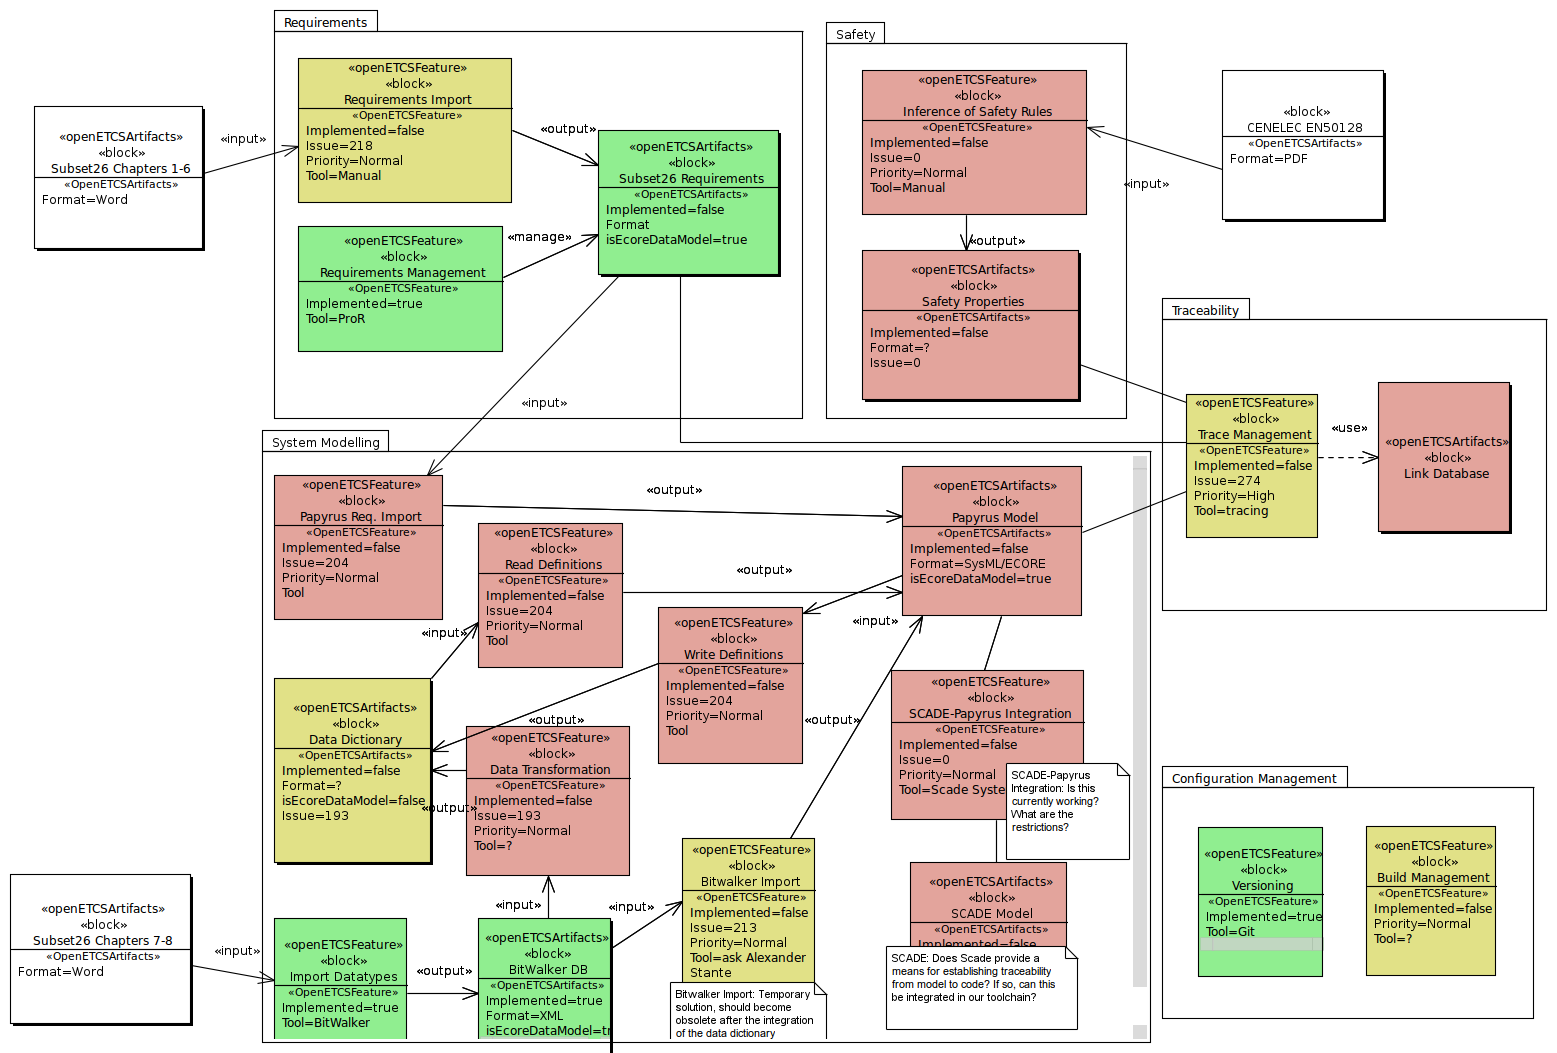
\includegraphics[width=\textwidth]{ToolChainmodel}
\caption{\label{fig:overview} Tool Chain overview (20.02.14) -- \\
  Green Block: Implemented \\
  Yellow Block: Work in Progress \\
  Red Block: Not started \\
  White Block: External Artifacts} 
\end{figure}

This block diagram is intended to grow according to the new feature request and the
needs of openETCS participants.  This diagram should be kept updated
as a reference of our tool chain, in any case the complete information
regarding the features availabilities  may be found in the eclipse product
definition.

Each feature of the toolchain is a block with the profile openETCsFeature"
and  each artifact is block with the profile openETCsArtifact''.  Each
feature realizes at least one use case and is implemented by at least
one tool. Note that in the tool platform feature  may also be
implemented as plug-ins.  The diagram also represents the order
also shows which tasks maybe done
in parallel and which ones are dependent of other tasks, but it does
not highlight neither the use of the tools, nor the order of actions
to be performed. This diagram should be completed by a guidelines on
how to use the tool chain and/or an activity diagram.

To mitigate the qualification process, we will first consider more
that one feature at a time considering that errors from a tool A may
be detected by a Tool B in the next step of the tool chain process.
Furthermore, the toolchain is a collection
of feature and not tools, this differs from Asplund and al. in the sense that
some of the tool integration mechanism that automates transformation of data, are part
of the feature and are not falling out of the scope of the qualification.

Due to our development process, a ``pre-qualification'' of tools should be made
when integrating a tool.

\marginpar{This high-level list should be detailed.}
\paragraph{Tool Integration Process for Qualification}

\begin{itemize}
\item Define name and version
\item Describe use cases
\item Provides justification of the tool within the tool chain
\item Provide input/output artifacts format (associated with the
  version)
\item Integrate the tool in the SysML model
\item Provide tool manual and other available documentation (associated with the version)
\item Link with an issue tracker
\end{itemize}

One possible implementation is to represent all these in formations
directly in the SysML model.

\marginpar{This high-level list should be detailed.  What I would expect: Which artefacts exist; How they are connected; When artefacts have to be re-validated (e.g. due to changes); What roles exist; who is responsible for what; etc.}
\paragraph{The Qualification Process}

\begin{enumerate}
\item Feature Analysis
  \begin{itemize}
  \item This step should assign a class to each feature based on the use cases.
  \item Define the potential errors
  \item Identify counter measure and/or error detection
  \item For T3 tools 2 alternatives:  certified compiler/generator or
    object code checker and/or exhaustive tester
  \end{itemize}
\item Tool platform  analysis 
  \begin{itemize}
  \item Provide evidence of the safety-goals mentioned in the
    previous sub-section
  \end{itemize}
\item Toolchain Analysis
  \begin{itemize}
  \item Defines the work-flow
  \item Identify the ``hot spots'' of the toolchain
  \item Rearrange the toolchain if possible
  \item Find new measures when needed with combining tools (redundancy with orthogonal
    codes \ldots{})
  \end{itemize}
\item Toolchain qualification verification 
  \begin{itemize}
  \item Check consistency of tool version with  manuals and other
    provided feature information
  \item Generate table to  check if all possible errors has a
    detection or a correction mechanism
\item Generate the qualification report
  \end{itemize}

\end{enumerate}

%%% Local Variables: 
%%% mode: latex
%%% TeX-master: "oetcs_qualification_process"
%%% End: 
